\section{Differenza tra paddr\_t e vaddr\_t}

\begin{itemize}
  \item \textbf{paddr\_t}:  indirizzo reale nella memoria RAM, gestito dal \textbf{kernel} e non accessibile dal processo utente.
  \item \textbf{vaddr\_t}: indirizzo virtuale, indirizzo che un \textbf{processo o il kernel} usa per accedere alla memoria. Deve essere \textbf{tradotto} tramite \textbf{tabella delle pagine} in un \verb|paddr_t|.
        ogni processo ha il proprio spazio di indirizzamento, lo stesso \verb|vaddr_t| può mappare diversi \verb|paddr_t| in diversi processi
\end{itemize}

Il processo usa una \verb|vaddr_t| e il SO, tramite \textbf{page table}, la traduce in \verb|paddr_t|.

\section{Overview}

\begin{itemize}
  \item \textbf{./config HELLO}: chiede quale configurazione utilizzare HELLO, DUMBVM. Genera una cartella dentro \verb|kern/compile| con il nome della config scelta
  \item \textbf{bmake depend}: analizza dipendenze tra i file sorgenti e gli header
  \item \textbf{bmake}: compila il kernel
  \item \textbf{bmake install}: installa il kernel compilato
\end{itemize}

\subsection{Generazione opzioni nel kernel}

Per abilitare o disabilitare funzionalità nel kernel come \verb|hello()|, si usano le \textbf{opzioni di configurazione}.

\paragraph{Esempio di attivazione opzione HELLO}

\begin{enumerate}
  \item Nel file \verb|conf.kern| va aggiunta la riga \verb|defoptions HELLO|. Questo dice al build che c'è un opzione chiamata HELLO
  \item Usare \verb|optfile HELLO main/hello.c| per dire al compilatore  compila il file solo se l'opzione HELLO è attiva
  \item Dopo aver eseguito \verb|./config HELLO|, verrà generato un file in \verb|compile/HELLO/opt-hello.h| nel quale sarà presente la riga
        \verb|#define OPT_HELLO 1| oppure commentata
  \item Puoi usare \verb|#include "opt-hello.h"| nei file per codice condizionale \verb|#if OPT_HELLO ... #endif|
\end{enumerate}

Questo permette all'interno del codice di abilitare o disabilitare porzioni di coidce in modo \textbf{condizionale}.

\section{Lab 1 - Modifica kernel}

OS161 è un SO che \textbf{gira su MIPS} simula e supporta l'esecuzione di programmi utente in formato ELF (Executable and Linkable Format).
Predilige la comprensibilità rispetto all'efficienza.

Troviamo: diver, scheduler base, thread gestiti dal kernel, traps e poco altro.
Da implementare: lock, syscall e sistema di memoria virtuale.

\subsection{Debug OS161}
Aprire due terminali: il primo in ascolto con \verb|sys161 -w kernel| e il secondo lancia
il debug con


\verb|ddd --debugger mips-harvard-os161-gdb kernel|.

\subsection{Threads e processi}

\textbf{Processo} programma in eseguzione con componenti quali \textbf{stack}, \textbf{heap}, \textbf{codice eseguibile}, \textbf{sezione dati} e \textbf{PC}.
Con \verb|fork()| si possono creare più istanze dello stesso programma.
\textbf{Thread} rappresenta un \textbf{flusso di esecuzione} all'interno di un processo. Ha associato un \textbf{stack}, \textbf{PC} e \textbf{registri}.


\begin{figure}[h!]
  \centering
  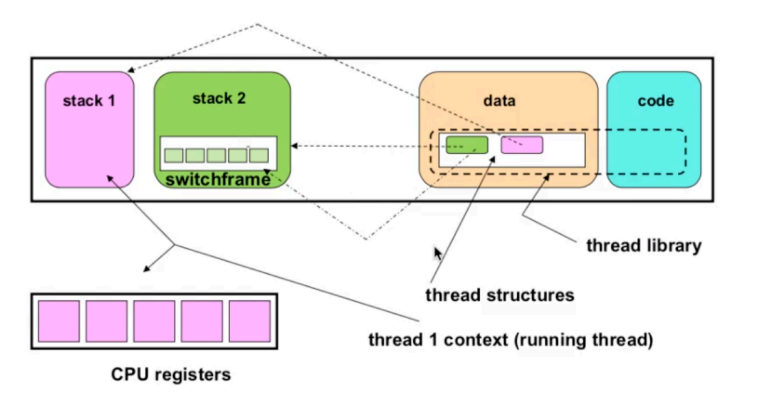
\includegraphics[width=0.5\linewidth]{content/OS_Internals/images/2026-06-03-13-22-41.png}
\end{figure}

I thread possono essere di due tipi: \textbf{user thread} e \textbf{kernel thread}.
Il \textbf{codice} e o \textbf{dati globali} sono condivisi tra thread.
Un thread è associato ad una \textit{struct}


\begin{minted}[breaklines]{c}
struct thread {
  char *t name;                               // Name of this thread.
  const char *t wchan_name;                   // Name of the wchan, if sleeping on
  threadstate t t state;                      // State         

  /* Thread subsystem internal fields. */
  struct thread_machdep t_machdep;            
  struct threadlistnode t_listnode;           
  void *t stack;                              // Kernel-level stack
  struct switchframe *t_context;              // Saved register context (on stack)  
  struct cpu *t_cpu;                          // CPU thread runs on 
  struct proc *t_proc;                        // Process thread belongs to

  //...
};
\end{minted}

\subsection{Funzioni principali}

\begin{itemize}
  \item \verb|thread_fork()|: crea un thread passando nome, processo padre, funzione da eseguire e relativi
  \item \verb|thread_yield()|: sospende il thread corrente senza terminarlo e passa la CPU ad un altro thread
  \item \verb|thread_exit()|: termina il thread corrente
\end{itemize}


\subsubsection{Come funziona \texttt{thread\_fork()}}

\begin{enumerate}
  \item Viene allocata una nuova struct thread tramite \verb|thread_create()|
  \item Inizializzato lo switchframe tramite \verb|switchframe_init()| che imposta i registri e il PC
  \item Invoca \verb|thread_make_runnable()| prende un thread e lo mette nella code dei \textit{ready} per essere schedulato
\end{enumerate}


\subsection{Processo utente}

Il processo utente include: \textbf{kernel}, \textbf{stack del processo}, \textbf{dati e codice dell'applicazione}, \textbf{i registri}.
Il kernel mantiene uno \textbf{stack separato} per l'esecuzione delle \textbf{syscall}.

La struttura che rappresenta un processo è chiamata \textbf{Process Control Block} (PCB) contenente info come:
\textbf{nome processo}, \textbf{spinlock}, \textbf{spazio di indirizzamento}, info sul File System.

\section{Lab 2 - Gestione della memoria}

Il sistema operativo ha due modi per  tradurre gli indirizzi logici a indirizzi fisici e viceversa:

\begin{itemize}
  \item Il kernel decide di \textbf{non effettuare} nessuna traduzione quando è in modalità kernel, utilizzando quelli fisici
  \item Utilizzare indirizzi logici per \textbf{kernel} e \textbf{utente}.
\end{itemize}

OS161 sceglie una versione intermedia: abilita la traduzione degli indirizzi logici in fisici \textbf{sia per kernel che per utente}.
Nel caso di un processore MIPS a 32 bit, lo spazio di \textbf{indirizzamento virtuale} è di 4GB diviso a metà tra kernel e utente.

Gli indirizzi riservati all'utente passano tramite \textbf{TLB} per velocizzare la traduzione.

Gli altri 2GB sono riservati al kernel così mappati:

\begin{itemize}
  \item 0.5GB: non mappato in TLB, si usa \textbf{relocation} che è una somma per tradurre indirizzi logici in fisici. Tenuta in cache.
  \item 0.5GB: non mappata in TLB, non mappata in cache perché usata per accedere ai dispositivi di I/O i quali sono lenti e lo scopo della cache è
        salvare dati, mentre se invio dati ad un dispositivo di I/O voglio ricevere un risultato
  \item 1GB: mappato in TLB ma non utilizzato.
\end{itemize}


\begin{figure}[h!]
  \centering
  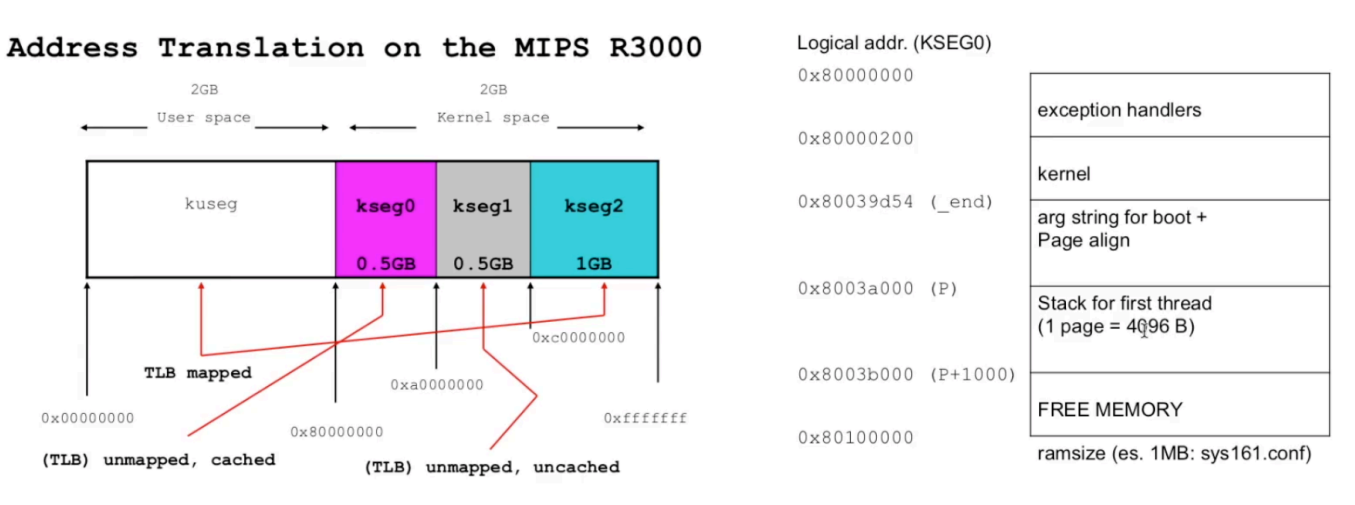
\includegraphics[width=0.6\linewidth]{content/OS_Internals/images/2026-05-31-15-37-48.png}
\end{figure}


\subsection{Allocazione della memoria per i processi}

Dopo aver assegnato lo spazio di indirizzamento ad un processo, il programma può essere avviato
in diversi modi:

\begin{itemize}
  \item Dal \textbf{kernel}
  \item Da un \textbf{processo utente}
  \item Da un \textbf{fork()}
\end{itemize}

Ogni ELF è composto da \textbf{segmenti}:

\begin{itemize}
  \item \textbf{segmento di codice}: .text, .rodata
  \item \textbf{segmento dati}: .data, .bss, .sbss
\end{itemize}

Non troviamo lo stack, in quanto è \textbf{dumbvm} ad allocare \textbf{12 pagine} in cima allo stack (\verb|0x7fffffff|).
L'indirizzo massimo di memoria fisica dipende dal sistema, ma l'\textbf{indirizzo virtuale} del primo spazio libero
è semrpe \verb|0x8003b000|.

A partire da quello di calcola l'indirizzo fisico corrispondente (firstpaddr) sottraendo
una costante chiamata \textbf{MIPS\_KSEG0}.

\subsubsection{\texttt{ram\_stealmem}}

Dumbvm usa allocazione \textbf{contigua} presa grazie a \verb|ram_stealmem()| la quale:

\begin{enumerate}
  \item riceve il numero di pagine, o frame, da allocare
  \item calcola la dimensione in byte: num-pagine * PAGE\_SIZE (4KB)
  \item somma questa dimensione a \textbf{firstpaddr}
  \item se il risultato supera l'ultimo indirizzo di RAM disponibile falllisce
  \item altrimenti restituisce l'indirizzo di partenza firstpaddr aggiornandolo.
\end{enumerate}

\subsubsection{getppages}

Per garantire l'assenza di \textbf{race condition} durante l'accesso alla memoria durante l'allocazione,
la funzione \verb|ram_stealmem| è protetta da un wrapper chiamato \verb|getppages()|.

La quale acquisisce un \textbf{spinlock} prima di chiamare \verb|ram_stealmem()| e lo rilascia subito dopo.

\begin{tcolorbox}
  \textbf{Spinlock:} Primitiva di sincronizzazione che \textbf{garantisce} l'accesso esclusivo a una sezione di codice
\end{tcolorbox}

Viene usata:

\begin{itemize}
  \item dal \textbf{kernel} tramite \verb|alloc_kpages| che alloca memoria per il kernel
  \item dall'utente tramite \verb|as_prepare_load|
\end{itemize}

\subsection{Rilascio della memoria}


\begin{flushleft}
  \begin{minipage}{0.65\linewidth}
    \raggedright
    Il rilascio della memoria non è presente di default, si può ovviare andando a basso livello in
    \verb|ram.c| oppure più agilmente in \verb|dumbvm|.

    \begin{enumerate}
      \item Aggiungere in \verb|dumbvm| una funzione \verb|freeppages()| complementare a \verb|getppages()| utilizzando una \textbf{bitmap} o una \textbf{freelist} tenute aggiorante ad ogni allocazione
      \item Sistema avanzato di gestione della memoria. Il Kernel continua con allocazione contigua, mentre si implementa la paginazione per i processi user
    \end{enumerate}
  \end{minipage}%
  \hfill
  \begin{minipage}{0.3\linewidth}
    \centering
    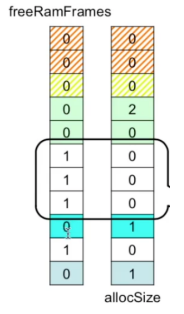
\includegraphics[width=0.5\linewidth]{content/OS_Internals/images/2026-05-31-16-10-30.png}  \end{minipage}
\end{flushleft}

Per implementare \verb|freeppages()|, servono alcune strutture dati fondamentali:

\begin{itemize}
  \item \verb|freeRamFrames|: \textbf{bitmap} tiene traccia di ogni frame (1 se libero, 0 se occupato), all'\textbf{avvio è tutto a 0} non ancora gestibile data la fase di bootstrap
  \item \verb|allocSize|: vettore che tine traccia del numero di pagine allocate
  \item \verb|nRamFrames|: rappresenta il numero totale di frame disponibili RAM
  \item uno \textbf{spinlock}: per proteggere la zona della \verb|free_mem|
  \item \textbf{allocTableActive}: indica se la fase di bootstrap è terminata
\end{itemize}

\subsection{System Call}

L'utente può richiedere funzionalità privilegiate al SO tramite \textbf{system call}.
Spesso l'utente non le chiama direttamente, ma tramite liberire di sistema le quali
forniscono un'interfaccia standard per tutti i vari sistemi operativi (es. \textbf{printf}).

Quando un programma esegue una syscall avviene un passaggio da user a kernel mode grazie ad una \textbf{trap},
eccezione controllata che \textbf{consente l'accesso al kernel in modo sicuro}.

Quando essa avviene il SO:

\begin{itemize}
  \item Salva lo stato del processo in \verb|trapframe|
  \item Questa struttura dati viene memorizzata nello stack kernel così da ripristinarla una volta conclusa la syscall
  \item Il \verb|System Call Handler| interpreta il numero della chiamata, repurta i parametri ed esegue il codice corrispondente alla richiesta
\end{itemize}

\section{Lab 3 - Sincronizzazione}

Nel contesto della programmazione concorrente si devono affrontare tre problematiche principali:

\begin{itemize}
  \item \textbf{Race condition}: il risultato dell'esecuzione dipende dall'ordine in cui i thread eseguono le istruzioni
  \item \textbf{Deadlock}: due o più thread si bloccano a vicenda aspettando risorse che non verranno mai rilasciate
  \item \textbf{Starvation}: un thread rimane bloccato perché altri thread a più altra priorità bloccano le risorse di cui ha bisogno
\end{itemize}

Per evitare ciò si devono utilizzare \textbf{primitiva di sincronizzazione} come \textbf{lock}, \textbf{semaphore} e \textbf{condition variable}.

\begin{tcolorbox}
  \textbf{Zona critica:} porzione di codice che deve essere eseguita in mutua esclusione
\end{tcolorbox}

Le strategie di sincronizzazione si basano sull'architettura e tre possibili scenari:

\begin{itemize}
  \item \textbf{Single core preemptive}: il SO può interrompere un thread in qualsiasi momento; necessssita di mutua esclusione
  \item \textbf{Single core non preemptive}: il thread in esecuzione non può essere interrotto; non necessita di mutua esclusione
  \item \textbf{Multi core}: esecuzione parallela e interruzioni; caso più complesso
\end{itemize}

\subsection{Peterson's solution}

\begin{minted}[breaklines]{c}
while (true) {
  flag[i] = true; // segnala l’intenzione di entrare
  turn = j; // cede il turno all’altro processo
  while (flag[j] && turn == j) {
  // attende finché l'altro vuole entrare ed è il suo turno
  }
  // ---- Zona critica ----
  // ...
  flag[i] = false; // uscita: segnala che non vuole più accedere
  // ---- Zona restante ----
}
\end{minted}

Il processo \textbf{i}:

\begin{enumerate}
  \item Dichiara di entrare nella zona critica impostando \verb|flag[i]| a true
  \item Cede il turno all'altro processo impostando \verb|turn = j|
  \item Attende finché l'altro processo (\textbf{j}) vuole entrare (\textbf{flag[j] == true}) ed è il suo turno
  \item Quando una delle condizioni non è più vera, entra nella zona critica
  \item Al termine reimposta \verb|flag[i] = false|
\end{enumerate}

Questo rispetta \textbf{mutua esclusione}, \textbf{progresso} e \textbf{attesa limitata}.

Tale soluzione non è affidabile su macchine moderne che implementano \textit{l'out of order execution}, e le cache
introducono ritardo.
Per questo è preferibile utilizzare primitive hardware come \textbf{test-and-set} o \textbf{compare-and-swap} o
meccanismi di sincronizzazione a livello di SO come \textbf{lock}, \textbf{semaphore} e \textbf{condition variable}.

\subsubsection{Memory barriers}

Primitive di basso livello che impongono ordine nell'accesso alla memoria.
Fondamentali in sistemi con modello di memoria \textbf{weakly ordered}. Si forza il processore
ad attendere che tutte le scritture precedenti siano completate e visibili prima di procedere con le successive.

\begin{tcolorbox}
  \textbf{Sistemi Strongly Ordered}: in questi sistemi dove le l'ordine delle operazioni di memoria è garantito, le barriere NON sono necessarie.
\end{tcolorbox}



\subsubsection{Istruzioni hardware}

\verb|Test-and-Set| e \verb|Compare-and-Swap| evitano \textbf{race condition} e letture \textbf{inconsistenti}.

La prima viene implementata con un ciclo \textbf{busy wait}.

\subsubsection{Atomic Variables}

Sono \textbf{interi} o \textbf{booleani} in cui accesso avviene in maniera \textbf{indivisibile}



\subsubsection{Semafori}

\begin{itemize}
  \item \textbf{Counting Semaphore}: variabile che tiene traccia del numero di processi che possono accedere a una risorsa, si basa su \verb|wait()| (busy waiting) e \verb|signal()|
  \item \textbf{Binary Semaphore}: può assumere solo i valori 0 e 1, spesso usato come mutex lock.
\end{itemize}

Si preferisce implementare i semafori con \verb|block| e \verb|wakeup| invece di busy waiting per evitare spreco di CPU.

\textbf{I semafori possono essere rilascaiti da un altro processo diverso da quello che l'ha acquisito}

\begin{tcolorbox}
  \textbf{Preemption e single core}: per garantire la mutua esclusione basta disabilitare gli \textbf{interrupt}, \textbf{impedendo} di fatto la \textbf{preemption}.
\end{tcolorbox}


\subsubsection{Mutex Lock}

Offrono due metodo \verb|acquire()| e \verb|release()| il loro utilizzao comporta
\textbf{spesso busy waiting}, infatti i mutex lock implementati in questa maniera sono
chiamati \textbf{spinlock}.

Sono Implementati con semafori binari.

\begin{tcolorbox}
  \textbf{Vincolo di ownership:} A differenza dei semafori, il processo che acuisisce un mutex lock è l'\textbf{unico autorizzato a rilasciarlo}.
\end{tcolorbox}

Migliore dei semafori per:

\begin{itemize}
  \item \textbf{Maggiore sicurezza}: rispettano il concetto di \textbf{ownership}
  \item \textbf{Flessibilità}: sincronizzazione più fini
  \item \textbf{Efficienza}: entrambi possono causare busy waiting.
\end{itemize}



\subsubsection{Condition Variable}

Semplifica la sincronizzazioine tra thread rispetto all'uso di mutex + semafori.

Offrono tre operazioni:

\begin{itemize}
  \item \verb|cv_wait()|: mette il thread in attesa e rilascia in automatico il mutex
  \item \verb|cv_signal()|: sveglia un solo thread in attesa (il semaforo avvisa tutti)
  \item \verb|cv_broadcast()|: sveglia tutti i thread in attesa
\end{itemize}

Ogni CV è associata ad un mutex, il quale va acuisito prima di chiamare \verb|cv_wait()| e mantenuto durante l'attesa.
La \verb|cv_wait()| sospende e rilascai il lock, il quale verrà riacquisito automaticamente al risveglio del thread.


In OS161, le funzioni \verb|cv_signal()| e \verb|cv_broadcast()| richiedono il lock come parametro
per verificarne l'uso corretto.


\begin{tcolorbox}
  \textbf{Nota}: Si utilizza un ciclo while per verificare la condizione prima
  della \verb|cv_wait()| e dopo il risveglio, poiché la condizione potrebbe non essere
  più valida. L'uso dell'if è accettabile solo in contesti molto semplici
\end{tcolorbox}


\subsubsection{Wait Channel}


Simili alle CondVar ma si \textbf{basano su spinlock}, implicando \textbf{busy waiting}.
Pensati esclusivamente per \textbf{uso interno al kernel} con vincoli quali:

\begin{itemize}
  \item Non supporta \textbf{lock multipli}
  \item Può essere posseduto solo per \textbf{brevi periodi}
\end{itemize}

La funzione principale è \verb|wchan_sleep()| che riceve in input un puntatore alla
struttura \verb|wchan| e uno \textbf{spinlock}.

\begin{enumerate}
  \item Sospende il thread con \verb|thread_switch()|
  \item Rilascia lo spinlock
  \item Al risveglio riacquisisce il lock
\end{enumerate}

Comportamento analogo a \verb|cv_wait()|, ma adattato all'ambiente kernel.

\subsubsection{Implementazione delle primitive in OS161}

\paragraph{Lock con semafori}

Utilizzo di un semaforo binario, facile ma non ideale per l'efficeinza.

\paragraph{Lock con Wait Channel e Spinlock}

Utilizzo di un \textbf{wait channel} per la sospensione e uno \textbf{spinlock} per
l'accesso sicuro alla struttura interna.

Deve includere il concetto di ownership, solo i thread che acquisisce il lockpuò rilasciarlo.
Per questo è necessario salvare un puntatore al \textbf{thread owner} con \verb|curthread|.


\paragraph{Lock}

\begin{itemize}
  \item \verb|lock_create(const char *name)|: crea un nuovo lock implementato usando un \textbf{semaforo binario} o un \textbf{wait channel}. Viene inizializzato uno \textbf{spinlock} interno per garantire l'accesso concorrente alle variabili interne del lock
  \item \verb|lock_destroy(struct lock *lock)|: libera risorse associate al lock (spinlock, semaforo/wait channel, memoria)
  \item \verb|lock_acquire(struct lock *lock)|: acquisisce il lock e a seconda della configurazione richiama le funzioni
  \item \verb|lock_release(struct lock *lock)|: rilascia il lock che il thread \textbf{possiede}
  \item \verb|lock_do_i_hold(struct lock *lock)|: Questa funzione verifica se il thread chiamante è il proprietario corrente del lock
\end{itemize}

\paragraph{CondVar}

\begin{itemize}
  \item \verb|cv_create(const char *name)|: Crea e inizializza una nuova condition variable (wait channel e spinlock)
  \item \verb|cv_destroy(struct cv *cv)|: dealloca la cv
  \item \verb|cv_wait(struct cv *cv, struct lock *lock)|
  \item \verb|cv_signal(struct cv *cv, struct lock *lock)|
  \item \verb|cv_broadcast(struct cv *cv, struct lock *lock)|
\end{itemize}

\section{Lab 4 - syscall waitpid}

\textbf{waitpid} è una syscall che permette ad un processo padre di attendere la terminazione di un processo figlio tramite \textbf{PID}.

Quando un processo termina, non viene immedatamente distrutto: se nessun processo ha ancora chiamato waitpid
per attendere la sua fine, il processo rimane in stato "zombie", ovvero la sua
struttura dati ( \verb|struct proc| ) resta allocata in memoria finché un altro processo non
ne recupera lo stato di uscita tramite waitpid .





\begin{flushleft}
  \begin{minipage}[t]{0.45\linewidth}
    \raggedright
    \subsection{\texttt{common\_prog() con proc\_wait()}}

    Questa funzione è una funzione \textbf{internal al kernel}, non è una syscall.
    Utile come prima versone più semplice, usata nel kernel perché solo in \textbf{kernel-space} si
    può accedere al puntatore \textbf{proc}.



  \end{minipage}%
  \hfill
  \begin{minipage}[t]{0.45\linewidth}
    \raggedright
    \subsection{\texttt{common\_prog() con sys\_waitpid()}}

    L'attesa avviene con una syscall, come farebbe un utente, in questo caso, non avendo \textbf{proc}, si deve
    lavorare con \textbf{PID}.
  \end{minipage}
\end{flushleft}


\begin{center}
  \begin{minipage}[t]{0.45\linewidth}
    \centering
    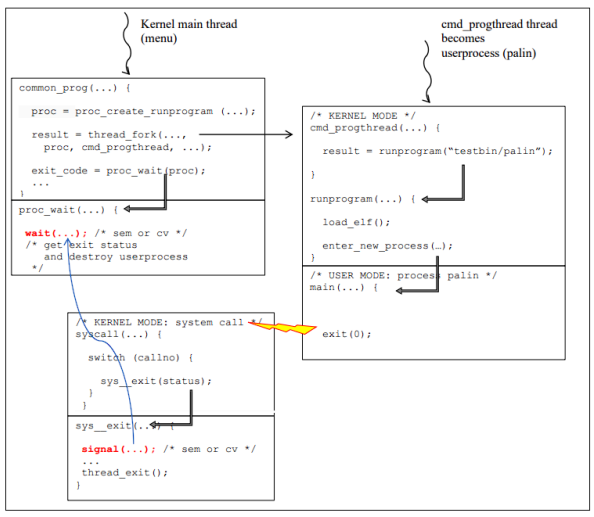
\includegraphics[width=\linewidth]{content/OS_Internals/images/2026-05-31-19-27-01.png}
  \end{minipage}%
  \hfill
  \begin{minipage}[t]{0.45\linewidth}
    \centering
    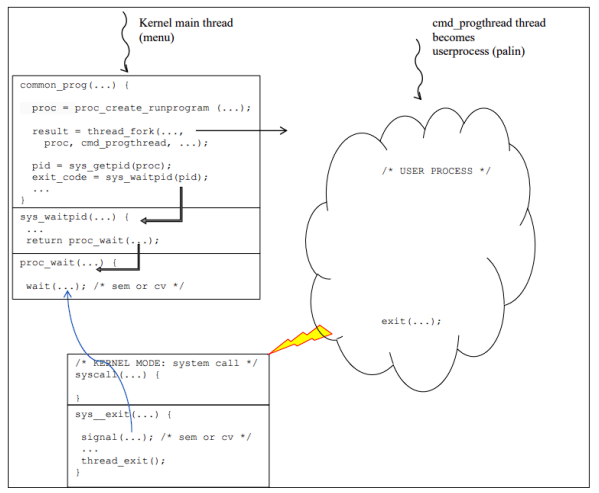
\includegraphics[width=\linewidth]{content/OS_Internals/images/2026-05-31-19-27-22.png}
  \end{minipage}
\end{center}


\begin{itemize}
  \item \verb|sys__exit(int status)|: permette ad un processo di terminare in modo ordinato
  \item \verb|sys_waitpid(pid_t pid, userptr_t statusp, int options)|: Questa funzione implementa la chiamata di sistema \verb|waitpid()|, che serve al
        processo padre per attendere la terminazione di un processo figlio.
  \item \verb|static struct _processTable|: Struttura globale che rappresenta la tabella dei processi per supportare waitpid
        e exit
  \item \verb|struct proc * proc_search_pid(pid_t pid)|: Restituisce un puntatore alla struttura proc associata a un determinato pid .
  \item \verb|static void proc_init_waitpid(struct proc *proc, const char *name)|: Inizializza i campi della struct proc necessari per il supporto a waitpid : assegna
        un PID, registra il processo nella tabella globale, e inizializza le primitive di
        sincronizzazione ( semaphore oppure condition variable + lock ).
  \item \verb|static void proc\_end\_waitpid(struct proc *proc)|: Rimuove un
        processo dalla tabella dei processi e dealloca le strutture usate per la
        sincronizzazione waitpid .
  \item \verb|static struct proc * proc\_create(const char *name)|: Crea una
        nuova struttura proc e la inizializza parzialmente.
  \item \verb|void proc_remthread(struct thread *t)|: Rimuove un thread da un processo. Usata quando un thread termina.
  \item \verb|int proc_wait(struct proc *proc)|: Questa funzione consente a un processo padre di attendere la terminazione di
        un processo figlio e di recuperarne lo stato di uscita.
\end{itemize}



